\begin{twocolumnfigure}[p]

\begin{fitheight}{5.2\standardhexwidth}
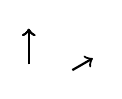
\begin{tikzpicture}
    \setfiguresize{-2.6}{-2.6}{+2.6}{+2.6}
    \begin{scope}
        \drawevenhexgrid{-2}{-2}{5}{5}
        \drawdashedcounter{+0.00}{-2.00}{0}
        \drawdashedcounter{+0.00}{-1.00}{0}
        \drawaircraftcounter{+0.00}{+0.00}{90}{F-4}{}{}
        \drawaircraftcounter{+1.00}{+0.50}{90}{F-4}{}{}
        \drawdashedcounter{+1.00}{+1.50}{0}
        \begin{scope}[shift={(-0.25,+0.25)},thick,->]
            \miniathex{+0.00}{-2.00}{\draw (90:0.0) -- (90:0.45);}
            \miniathex{+0.00}{-1.00}{\draw (90:0.0) -- (90:0.45);}
            \miniathex{+1.00}{+0.50}{\draw (90:0.0) -- (90:0.45);}
        \end{scope}
        \miniathex{+0.00}{+0.00}{\draw [thick,->] (30:0.35) -- (30:0.65);}
     \end{scope}
\end{tikzpicture}
\end{fitheight}
\hfil
\begin{fitheight}{5.2\standardhexwidth}
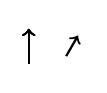
\begin{tikzpicture}
    \setfiguresize{-2.6}{-2.6}{+2.6}{+2.6}
    \begin{scope}[rotate=90]
        \drawevenhexgrid{-2}{-2}{5}{5}
        \drawdashedcounter{-2.00}{+0.00}{0}
        \drawdashedcounter{-1.00}{+0.00}{0}
        \drawaircraftcounter[90]{+0.00}{+0.00}{0}{F-4}{}{}
        \drawaircraftcounter[90]{+1.00}{-0.50}{0}{F-4}{}{}
        \drawdashedcounter{+2.00}{-0.50}{0}
        \begin{scope}[shift={(+0.20,+0.30)},thick,->]
            \miniathex{-2.00}{+0.00}{\draw (0:0.0) -- (0:0.45);}
            \miniathex{-1.00}{+0.00}{\draw (0:0.0) -- (0:0.45);}
            \miniathex{+1.00}{-0.50}{\draw (0:0.0) -- (0:0.45);}
        \end{scope}
        \miniathex{+0.00}{+0.00}{\draw [thick,->] (330:0.35) -- (330:0.65);}
        %\begin{scope}[shift={(0.0,+0.5)},anchor=east]
        %    \miniathex{-2.00}{+0.00}{\draw node {\minitable{r}{preparatory\\ HFP}};}
        %    \miniathex{-1.00}{+0.00}{\draw node {\minitable{r}{preparatory\\ HFP}};}
        %    \miniathex{+0.00}{+0.00}{\draw node {\minitable{r}{start\\ position}};}
        %    \miniathex{+1.00}{-0.50}{\draw node {\minitable{r}{slide\\ execution}};}
        %    \miniathex{+2.00}{-0.50}{\draw node {\minitable{r}{next\\ HFP}};}
        %\end{scope}
    \end{scope}
\end{tikzpicture}
\end{fitheight}
\hfil
\begin{fitheight}{5.2\standardhexwidth}
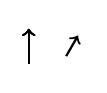
\begin{tikzpicture}
    \setfiguresize{-2.6}{-2.6}{+2.6}{+2.6}
    \begin{scope}[rotate=90]
        \drawoddhexgrid{-2}{-1.5}{5}{5}
        \drawdashedcounter{-2.00}{+0.00}{0}
        \drawdashedcounter{-1.00}{+0.00}{0}
        \drawaircraftcounter[90]{+0.00}{+0.00}{0}{F-4}{}{}
        \drawaircraftcounter[90]{+1.00}{-0.50}{0}{F-4}{}{}
        \drawdashedcounter{+2.00}{-0.50}{0}
        \begin{scope}[shift={(+0.20,+0.30)},thick,->]
            \miniathex{-2.00}{+0.00}{\draw (0:0.0) -- (0:0.45);}
            \miniathex{-1.00}{+0.00}{\draw (0:0.0) -- (0:0.45);}
            \miniathex{+1.00}{-0.50}{\draw (0:0.0) -- (0:0.45);}
        \end{scope}
        \miniathex{+0.00}{+0.00}{\draw [thick,->] (330:0.35) -- (330:0.65);}
    \end{scope}
\end{tikzpicture}
\end{fitheight}

\x{
\figurecaption{figure:slide-maneuvers}{Slide Maneuvers}
}{
\figurecaption{figure:slide-maneuvers}{Slides to the right, each preceded by two preparatory HFPs and followed by another HFP. The execution of the slide is indicated by the counter images with solid borders. The number of preparatory HFPs required depends on the aircraft speed and other factors. The execution of a slide is identical to that of a displacement roll, although other aspects are different.}
}

\end{twocolumnfigure}
